\section{Phylogenetic Reconstruction}

% 1/10 mutation rate, .0002 bit mutaiton rate
Each sampled specimen genome has 35 64-bit event tags, under a net bitwise point-mutation rate per generation of 0.00002.

The point-mutation distance between tags was calculated using a pairwise Hamming metric.
These distances were stored as a matrix \ref{phylo_distance_matrix_heatmap}, along with the phenotype categories for each stint.

To generate the phylogenetic tree \ref{phylo_nj_tree}, the distance matrix was transformed to a lower-triangular matrix, and then fed to BioPython's \texttt{Bio.Phylo.TreeConstruction.DistanceMatrix()} constructor, along with the Neighbor Joining clustering method.
The non-terminal branch lengths were adjusted to equal the average branch length of their children.
Terminal nodes were then sorted by time (lowest stint first) with respect to their sibling nodes.
Each parent of a subtree was then assigned the value of the lowest child and then also sorted across its siblings.
This was repeated until reaching the root node.

The parsimony tree was built using BioPython's \texttt{Phylo.TreeConstruction.ParsimonyTreeConstructor}, using the default \texttt{Phylo.TreeConstruction.ParsimonyScorer} scorer along with the Nearest Neighbor Interchanges searcher.
In conformance to the \texttt{phylip} format, stint tags were `aligned' by concatenation across stints, and stint IDs were padded up to length 10 with left-leading zeros.
The tree-finding algorithm was then executed until an optimal solution was found.
Since stints 0 and 1 are outliers, the parsimony tree was stored both with them and without them, rerooted at stint 2.

The SciPy linkage tree \ref{phylo_scipy_linkage_tree} was generated using SciPy's \texttt{scipy.cluster.hierarchy.linkage} function with default arguments.
This was then converted into a DendroPy tree, which in turn was converted into an ALife dataframe.
The ALife dataframe was finally converted into a standard BioPython tree, which was then sorted using the sibling method, and stored.

All trees were drawn unsorted, sorted, and ladderized using BioPython's \texttt{ladderize} method.
These drawings were generated both with and without `outlier' nodes (stints 0 and 1).

\begin{figure*}
\centering
\includegraphics[width=0.8\linewidth]{{submodule/dishtiny_event_tag_phylogenetics/teeplots/phylo_tree_no_outliers/viz=draw+ext=}}

\caption{
TODO
}
\label{fig:phylo_nj_tree}
\end{figure*}

\begin{figure*}
\centering
\includegraphics[width=0.8\linewidth]{{submodule/dishtiny_event_tag_phylogenetics/teeplots/scipy_linkage_tree_no_outliers/viz=draw+ext=}}

\caption{
Phylogeny of sampled focal strain representatives across stints reconstructed using hierarchical clustering algorithm \citep{virtanen2020scipy}.
Each leaf node corresponds to a sampled representative.
Representatives from stints 0 and 1, which share no common ancestry with representatives from other stints, are excluded.
Numbers refer to stint that each representative was sampled from.
Color coding and parentheticals of stint labels correspond to qualitative morph codes described in Table \ref{tab:morph_descriptions}.
}
\label{fig:phylo_scipy_linkage_tree}
\end{figure*}

